\documentclass{beamer}


% \usepackage{CJKnumb}\usepackage{beamerthemesplit}

\mode<article>
{
  \usepackage{beamerbasearticle}
  \usepackage{fullpage}
  \usepackage{hyperref}
}

%\usepackage{beamerthemesplit} 
%\usepackage{beamerthemeshadow}  
%\usepackage[width=2cm,dark,tab]{beamerthemesidebar}


% Setup appearance:

%\usetheme{Darmstadt}
\usefonttheme[onlylarge]{structurebold}
\setbeamerfont*{frametitle}{size=\normalsize,series=\bfseries}
\setbeamertemplate{navigation symbols}{}

\renewcommand\arraystretch{1.5}

% Standard packages

\usepackage[english]{babel}
%\usepackage[latin1]{inputenc}

\usepackage{epsf}
\usepackage{amsmath,amssymb}
\usepackage{graphicx}
\usepackage{tabularx}

% \usepackage[usenames,dvipsnames]{color}
\definecolor{shadow}{gray}{0.8}
\newcommand{\redc}[1]{{\color{red} #1}}
\newcommand{\bluec}[1]{{\color{blue} #1}}
\newcommand{\shadowc}[1]{{\color{shadow} #1}}
\definecolor{myyellow}{HTML}{FFB700}
\newcommand{\yellowc}[1]{{\color{myyellow} #1}}
\newcommand{\greenc}[1]{{\color{green} #1}}
\renewcommand{\v}[1]{\textbf{\textit{#1}}}
\renewcommand{\d}[1]{\textrm{#1}}


\usepackage{amsfonts}
\newcommand{\tickYes}{\checkmark}
\usepackage{pifont}
\newcommand{\tickNo}{\hspace{1pt}\ding{55}}

% \usetheme{Boadilla}
% \usetheme{Copenhagen}
% \usetheme{Madrid}
\usetheme{Singapore}


\begin{document}
%\title{Comparative atomistic and coarse-grained study of water: Simulation details vs. Simulation feasibility}
%\title[Optimizing SPME]{Optimizing Working Parameters of the Smooth Particle Mesh Ewald Algorithm}
\title[]{
  Estimating the force computation error in inhomogeneous and correlated
  molecular systems
}
%
\author{Han Wang}
\institute[FUB] {
  Institute for Mathematics, Freie Universit\"at Berlin, Germany
\vskip 0.4cm
Joint with: Christof Sch\"utte (FUB), Pingwen Zhang (PKU)}
\date[12 Apr 2011]{12 Apr 2011}
\frame{\titlepage}

% \begin{frame}{Why?}
%   \begin{itemize}
%     \vfill
%   \item <1-> Why force computation?
%     \begin{itemize}\itemsep 3pt
%     \item <2->Molecular dynamics simulation.
%     \item <3->Computationally intensive: \redc{$ \sim 90 \%$}
%     \item <4->One of the main sources of the \redc{``error''}.
%     \item <5->May introduce \redc{unphysical artifacts}.
%     \end{itemize}
%     \vfill
%   \item <6-> Why error estimate?
%     \begin{itemize}\itemsep 3pt
%     \item <7->Understanding \& correcting
%       the unphysical artifacts, quantitatively.
%     \item <8->Correction to force, energy, pressure, etc.
%     \item <9->Boost the efficiency of simulation automatically.
%     \end{itemize}
%     \vfill
%   \end{itemize}
% \end{frame}


\begin{frame}{Overview of the error estimates}
  \begin{itemize}
    \vfill
  \item <1-> Why force computation is important?
    \begin{itemize}\itemsep 3pt
    \item Molecular dynamics simulation.
    \item Computationally intensive: \redc{$ \sim 90 \%$}
    \item One of the main sources of the \redc{``error''}.
    \end{itemize}
    \vfill
  \item<2-> Why error estimates?
    \begin{itemize}\itemsep 3pt
    \item Correction to \redc{force, energy, pressure, etc.}
    \item Boost the \redc{accuracy \& efficiency} of simulation automatically.
    \end{itemize}
    \vfill
  \item<3->   Current error estimates:
    \begin{itemize}\itemsep 3pt
    \item <3-> homogeneous  + uncorrelated \quad \bluec{\tickYes\:$\mathcal O(1)$}
    \item <4-> inhomogeneous  + uncorrelated \quad \redc{\tickYes\:$\mathcal O(N\log N)$}
    \item <4-> inhomogeneous  + correlated \quad \redc{\tickYes\:$\mathcal O(N^2\log N) \rightarrow \mathcal O(N\log N)$}
    \end{itemize}
    \vfill
  \end{itemize}
\end{frame}


\begin{frame}{Liquid-vapor equilibrium of Lennard-Jones particles}
  \begin{figure}
    \centering
    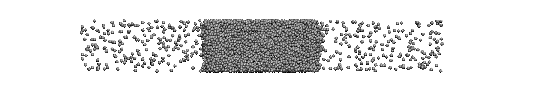
\includegraphics[scale=1]{figs/t0.85-n16000-rc07.5uni/confout-02.eps}\\
    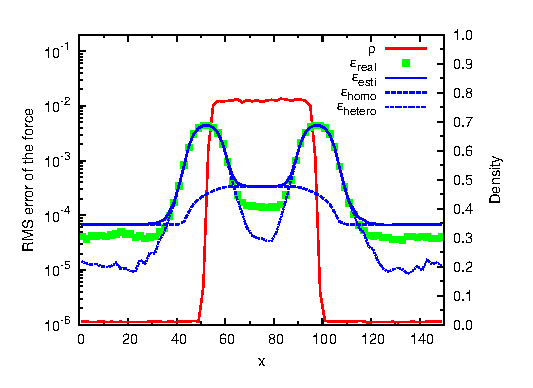
\includegraphics[]{figs/t0.85-n16000-rc07.5uni/error-uniform.eps}
  \end{figure}
\end{frame}



\end{document}
